\section{Structuur}
Deze sectie beschrijft de structuur van belangrijke en interessante onderdelen van het systeem. 
Deze beschrijvingen worden al dan niet ondersteund met een bijbehorend diagram indien dit van toepassing is.

\subsection{Leslokalen en vakken}
Volgend UML diagram beschrijft de structuur van de verscheidene klassen betreffende leslokalen en lessen die met elkaar gerelateerd zijn op het logisch niveau van het systeem.
Deze klassen bezitten data vanuit de databank die nodig zullen zijn om lessenroosters en examenroosters te plannen.

\begin{figure}[H]
	\centering
	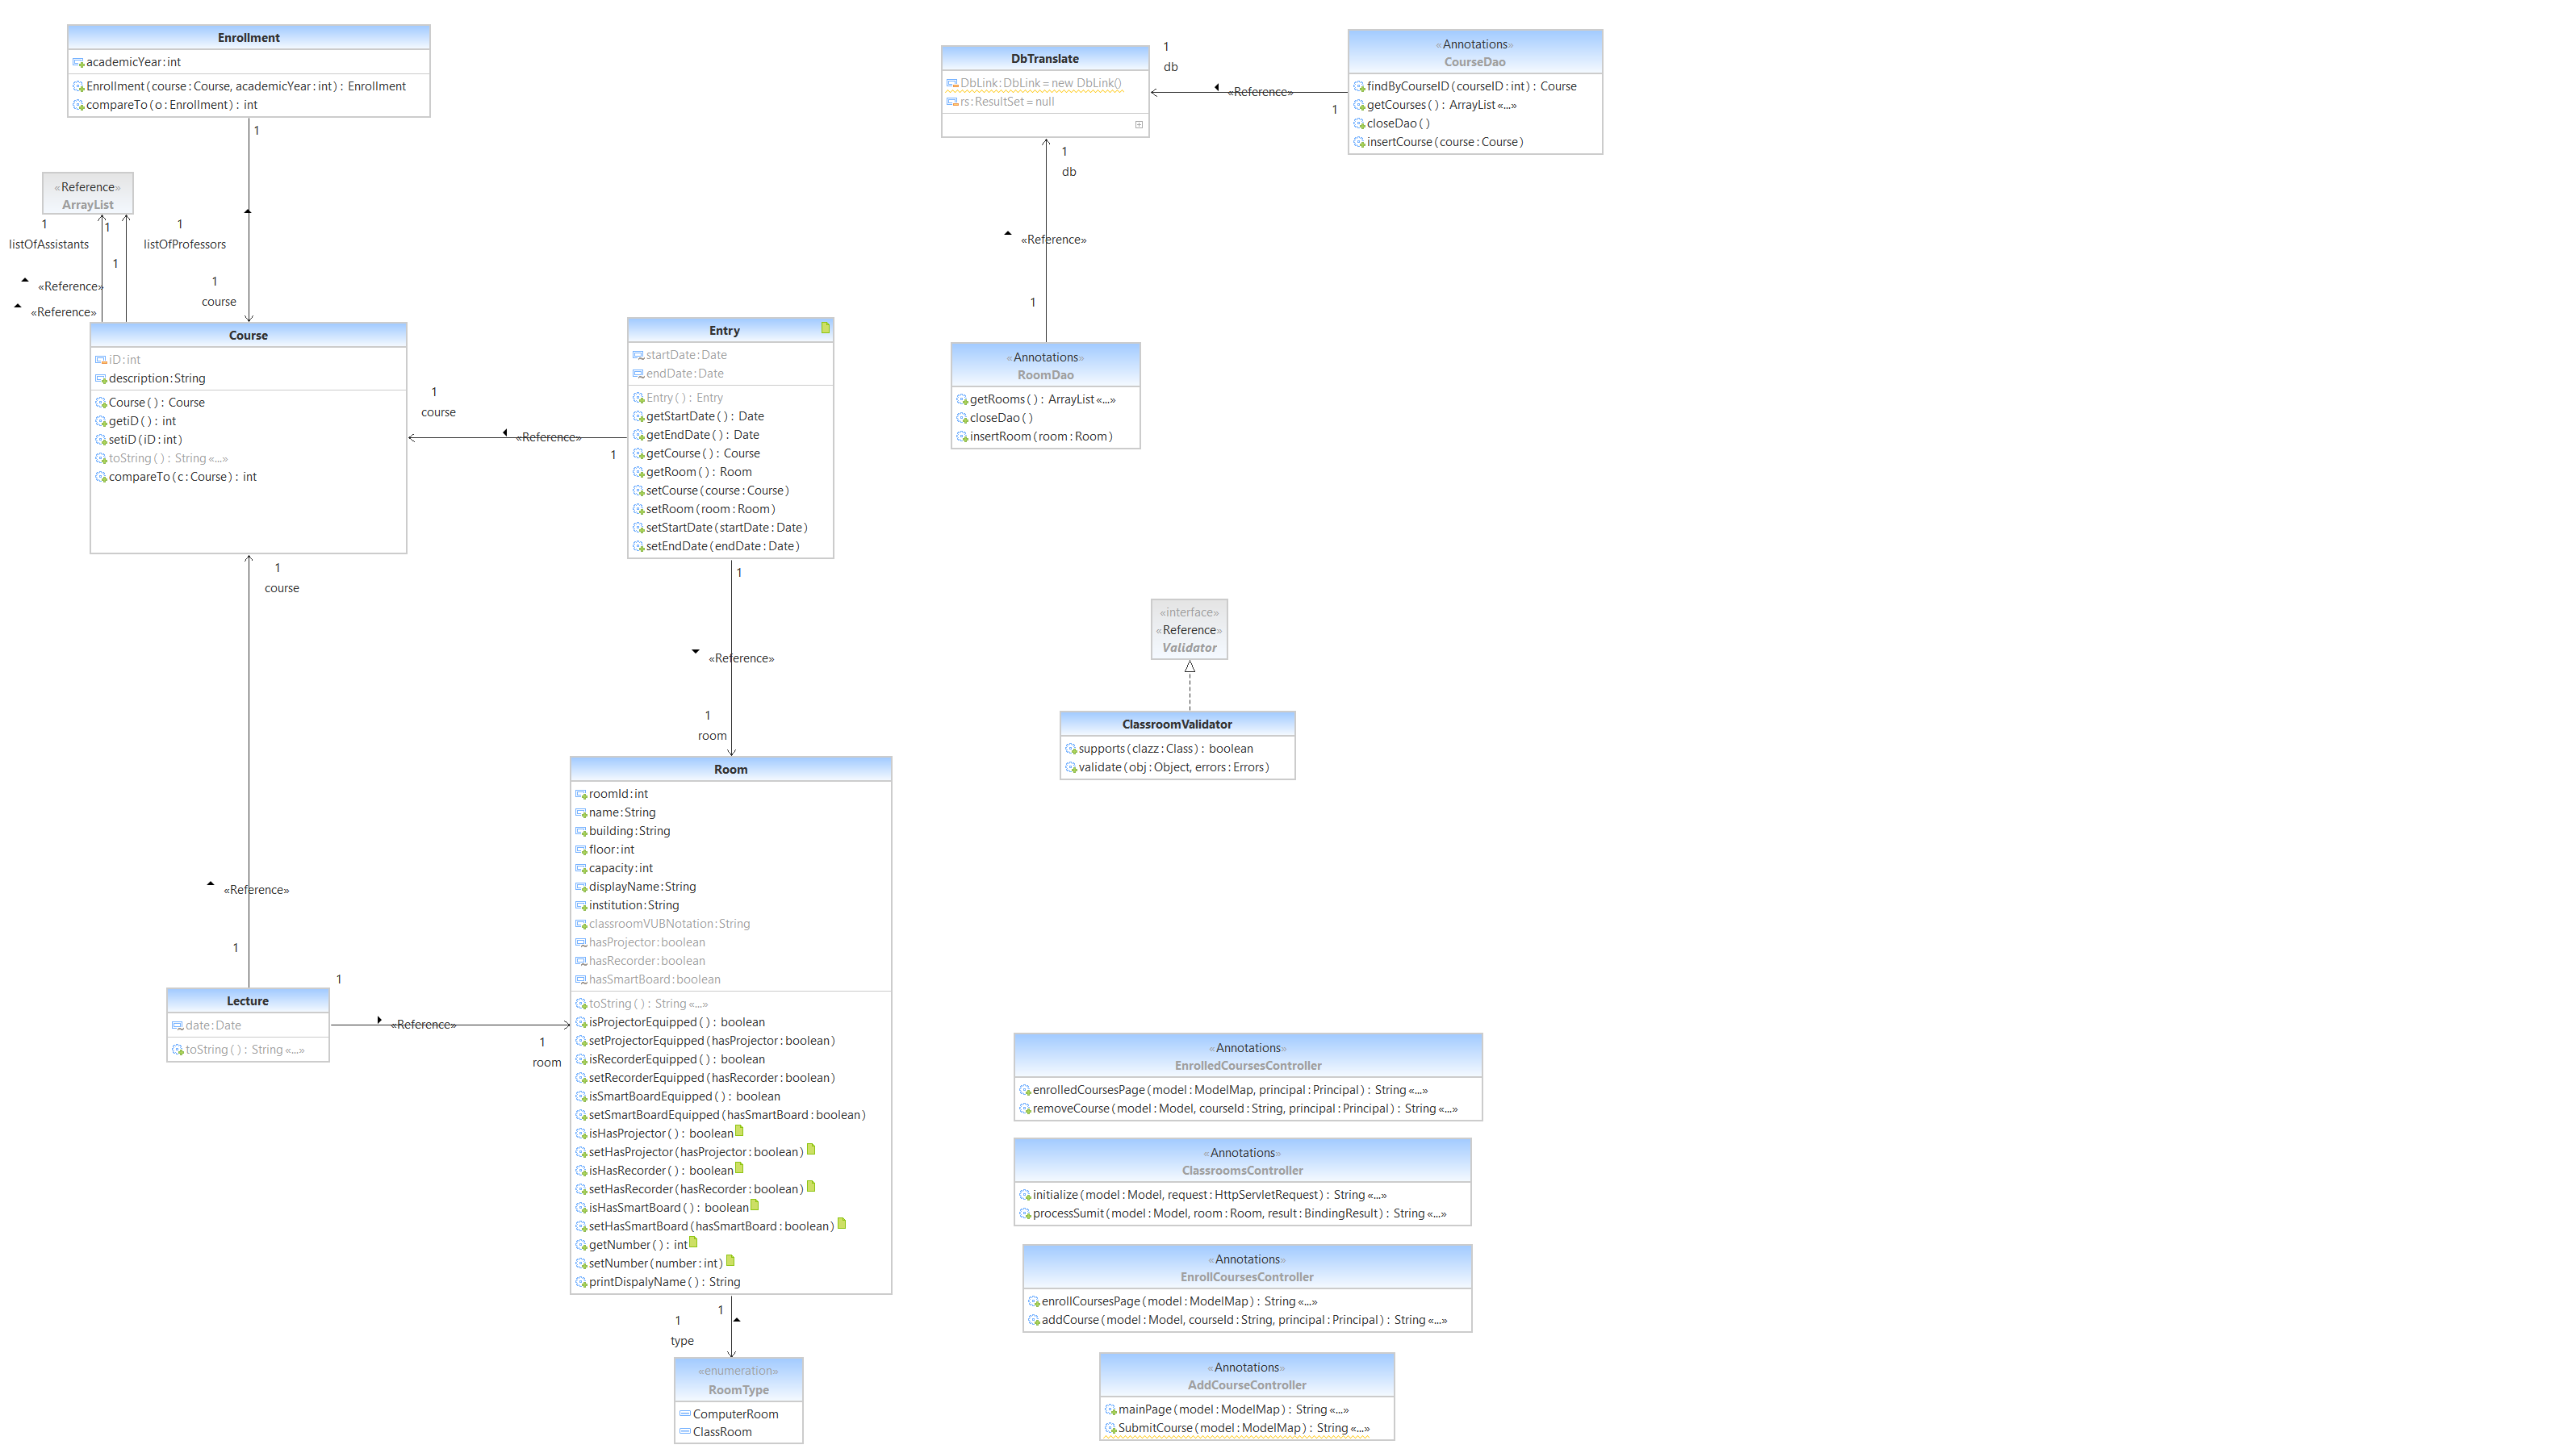
\includegraphics[scale=0.4]{img/roomsAndCourses}
	\caption{UML klassediagram voor leslokalen en vakken}
	\label{fig:roomsAndCourses}
\end{figure}

\subsection{Logging}
\label{subsec:logging}
Als logging framework werd gekozen voor SLF4J\cite{slf4j}.
Dit framework is echter een API die het maken van logs versimpelt voor de programmeur en vereist dus nog een geconfigureerde backbone.
Als backbone werd gekozen voor logback \cite{logback}.\\

In loggingsystemen kan men verschillende soorten logberichten produceren. 
Het systeem zorgt er dan voor dat deze berichten op de juiste plaats terecht komen.
De belangrijkste soorten berichten zijn: info, warning, error en debug.
In wat volgt wordt de configuratie van het loggingsysteem uitgeklaard.\\

Alle logberichten worden op de standaard output getoond.
Verder worden er specifieke logs opgeslagen naar bestanden.
Er zijn 2 folders voorzien voor logs: eentje voor debug logs en een folder met daarin een algemene log file.
Deze algemene log file bevat log berichten vanaf het niveau 'INFO', wat betekent dat het dus INFO, WARNING en ERROR logs bewaart.
Voor de debug logs wordt iedere dag een nieuwe file aangemaakt omdat het systeem een massa aan debug logs kan produceren op een dag.\\

Voor het in productie gaan van de applicatie is het sterk aangeraden de debug logs uit te schakelen daar het genereren van logs het systeem kan vertragen.

\subsection{Scheduler}
\label{subsec:scheduleclass}
Volgend UML klassediagram beschrijft de structuur van de klassen betreffende lessenroosters en het maken van zulke roosters.
Figuur \ref{fig:scheduling} beschrijft hoe het planningsprobleem in onze applicatie geformuleerd wordt.
Het framework OptaPlanner\cite{optaplanner} maakt gebruik van deze klassen door middel van annotaties om lessenroosters te maken.
Nu volgt een simpele beschrijving van de structuur.\\

Een \textit{Schedule} is een planning.
Zo een planning bestaat uit een sequentie van \textit{Entries}.
Een \textit{Entry} kan men vergelijken met een afspraak in een agenda.
In ons systeem wordt zo dus gevormd door een klaslokaal (Room), een vakonderdeel (CourseComponent) en een tijdstip (Date).
Een initialisatieklasse, \textit{SchedulerInitializer}, voorziet de beschikbare datums en tijdstippen.
Het verwezenlijken van een planning wordt opgelost door de klasse \textit{SchedulerSolver}.
Deze klasse zal gebruik maken van OptaPlanner om een \textit{ Schedule} te genereren.
Impliciet zal de SchedulerSolver gebruik maken van de klassen SchedulerHelper en EntryDifficultyComparator in een poging een zo goed mogelijk lessenrooster te bekomen.
Meer uitleg over hoe OptaPlanner werkt en geconfigureerd is wordt beschreven in  \ref{subsec:scheduling}.
 
\begin{landscape}
	\begin{figure}[H]
		\centering
		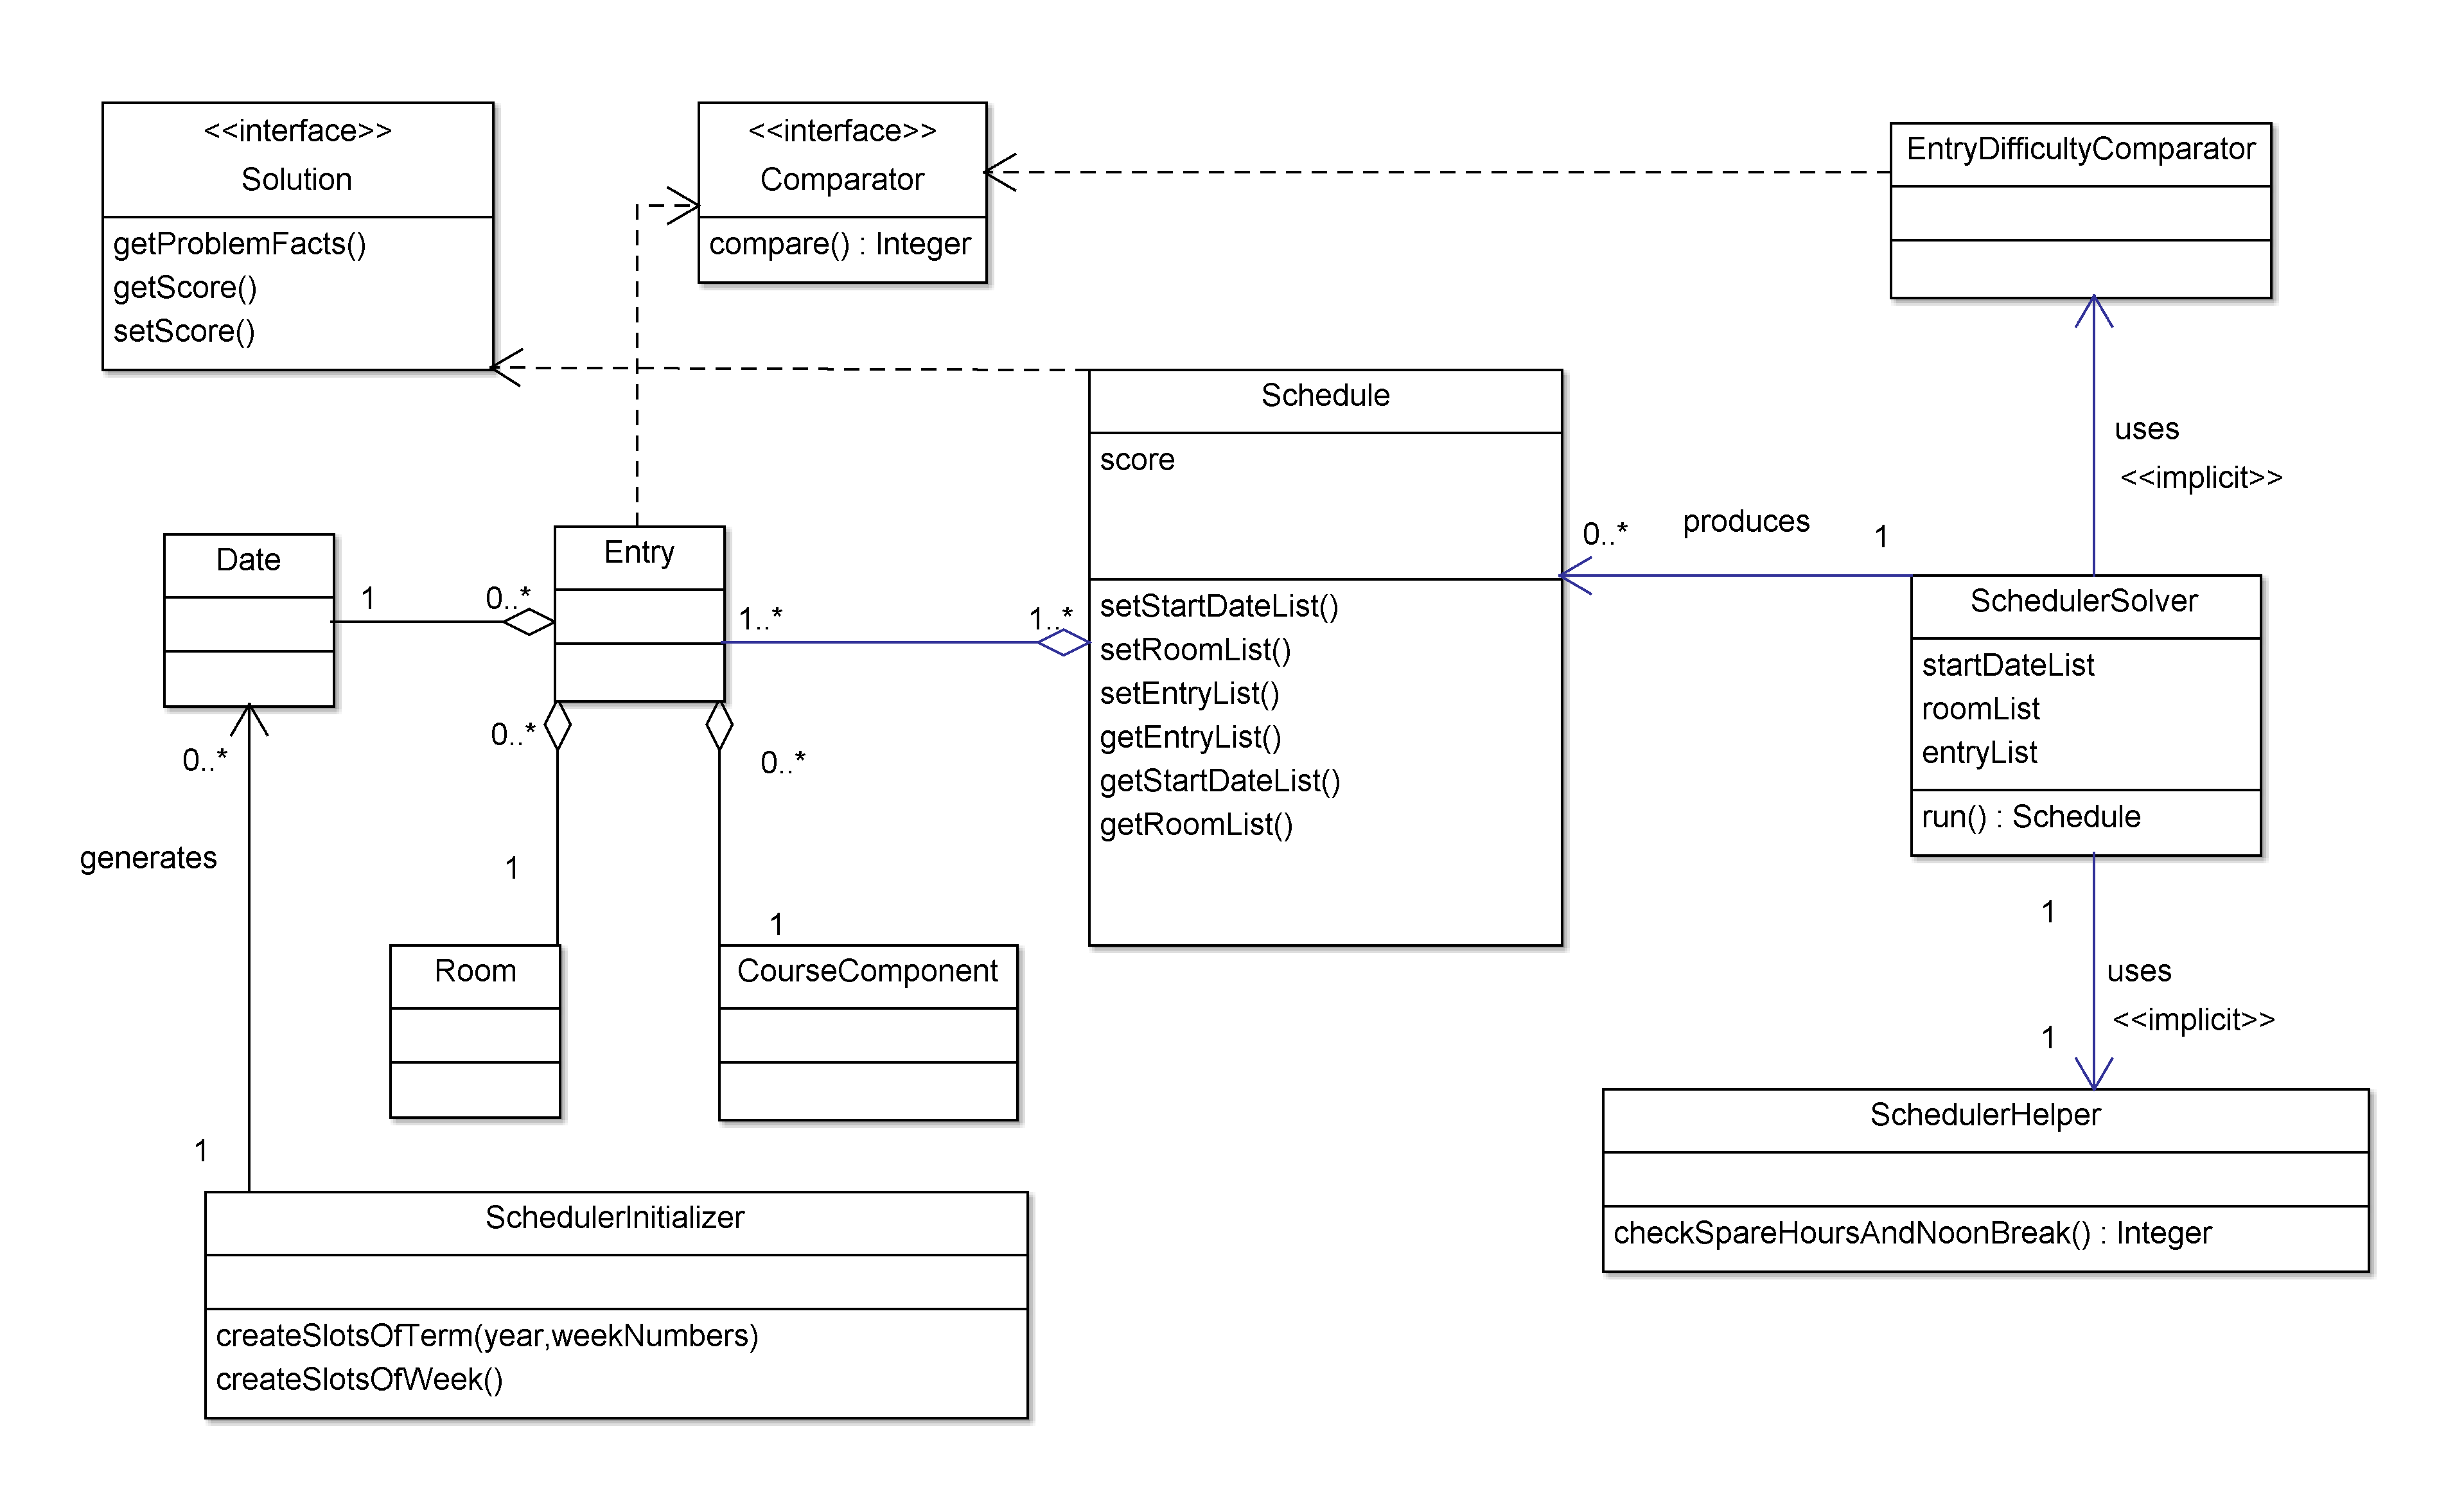
\includegraphics[scale=0.2]{img/scheduler}
		\caption{UML klassediagram voor scheduling}
		\label{fig:scheduling}
	\end{figure}
\end{landscape}
